% !TEX root = 0_main.tex
\chapter{Preliminaries and Background}
In this chapter,
-we provide general background information about secure multi-party computation
-we also introduce the generalized problem of secure function evaluation (SFE). and it two-party version and the threat model.
-Then we explain the Yao's Garbled Circuit protocol that enables two-party SFE for honest-but-curios adversary.
-We also explain the theoretical advancement and optimization on the protocol.
-Then we explain basics about combinational and sequential Boolean circuits.

\section{Secure Multi-party Computation}
the general problem of secure multi-party computation:
We have mutually suspicious parties that each has a private attribute (e.g., salary) and wish to compute a joint function (e.g., ) on their attributes.
They have to use some distributed protocol to evaluate and learn the output of the function without leaking their private information to other parties.
If we could find a third party that all the individuals trust, they could give her the inputs and she computes the function and returns the result to the parties.
Of course such a trusted party cannot be found in real scenarios of distributed systems.
Thus at best, we can emulate such a trusted third party with a cryptographic protocol~\cite{goldreich2013general}.
\fig{fig:multi-party-model} shows the idea model with a trusted third party and its emulation in a real model using a secure multi-party computation protocol.

\begin{figure}[ht]
    \centering
    \begin{subfigure}[tl]{0.35\textwidth}
        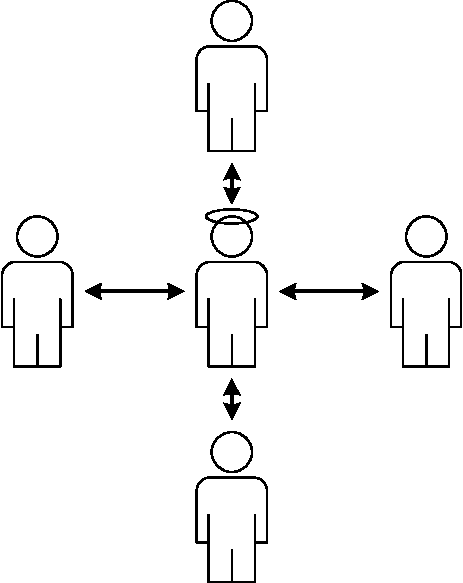
\includegraphics[width=\textwidth]{emulate_ideal-crop.pdf}
        \caption{Ideal Model}\label{fig:ideal-model}
    \end{subfigure}
		~~~~
    \begin{subfigure}[tr]{0.35\textwidth}
        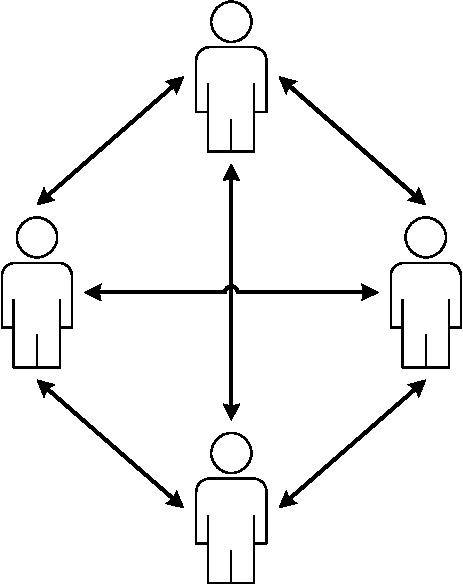
\includegraphics[width=\textwidth]{emulate_real-crop.pdf}
        \caption{Real Model}\label{fig:real-model}
    \end{subfigure}\\
    \caption{Emulation of a trusted third-party in secure multi-party computation (schematic based on~\cite{goldreich2013general}).}\label{fig:multi-party-model}
\end{figure}

Such emulation is possible under assumption about the emulation such as security level and type of the function that can be evaluated.
Initial general protocols Yao's Garbled Circuit Protocol GMW that are able to evaluate general functions.
Homomorphic encryption and Shamir's secret sharing are able to evaluate special function such as addition and multiplication.
In this thesis, we focus on the general secure multi-party computation where arbitrary desired function can be evaluated by the protocol.

\section{Secure Function Evaluation Definition}
The general secure multi-party computation is also known as secure function evaluation (SFE). It can be defined as follow: p parties each have an attribute: i1, ... ip. They want to compute function o = f(i1,i2, .. ip) where o is a tuple (o1, o2, ..., op) such that ok belongs to the kth party.
the function f can also be described as a tuple of functions f = (f1, f2, ...,  fp) where the output of fk(p1, p2, .. pm) = ok belongs to kth party.
(A common special case is that fi's are the same and all parties revives the same output. For example in case of the average of salaries, the result of the average function is evaluated and shared with all the participating parties).

\section{Two-Party Secure Function Evaluation}
two-party SFE is an important special case of general secure multi-party computation that was solved initially by Andrew Yao and GMW.
There are two parties Alice and Bob each has an input a and b and they want to compute (o1, o2) = (f1(a,b), f2(a,b)) where o1 belong to Alice and o2 belongs to Bob.

\begin{figure}[ht]
\centering
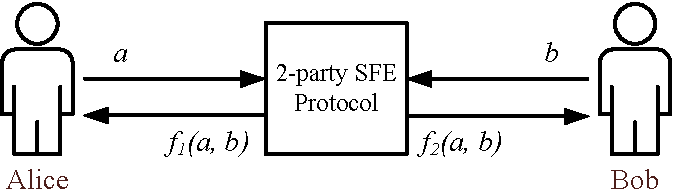
\includegraphics[width=0.70\textwidth]{two_party_SFE-crop.pdf}
\caption{The two-party secure function evaluation (SFE) protocol.}
\label{fig:globalflow}
\end{figure}

\section{Adversary Model}
We assume that all the parties are semi-honest which means that they follow the protocol exactly as specified without deviation or malicious behavior but they try to learn as much as possible about the other party's input from the information they receive during the protocol.
This model is often called honest-but-curious (HBC) adversary model in the literature and it is the basis for building a stronger security protocol.

In related work chapter \ref{ch:related}, we mention some of the recent approaches to extend the adversary model for two-party SFE to make it secure against the malicious adversary who can deviate from the protocol.

\section{Yao's Garbled Circuit Protocol}
Yao introduced the GC protocol for 2-party Secure Function Evaluation (SFE) in the 1980's \cite{yao1986generate}.
GC is described as a circuit whose wires carry a string valued-token instead of a bit.
Consider two parties, Alice and Bob, who want to evaluate a function $f(\cdot)$ without revealing their inputs to each other.
The function needs to be represented as a combinational Boolean circuit.
To begin with, we assume the circuit consists of a single gate with two input wires, $w_{a}$, $w_{b}$ and one output wire $w_{c}$.
Alice knows the value of input $w_{a}$ denoted by $v_{a}$ and Bob knows the value of input $w_{b}$ denoted by $v_{b}$.
The gate is also represented by a four-entry truth table $G[v_{a}, v_{b}]$.
There are two main phases in Yao's protocol.
First, Alice encodes or garbles the circuit by generating garbled tables.
Second, Bob evaluates the output denoted by $v_{c}$ without knowing anything about $v_{a}$ other than what can be deduced from the output and his own input.

The steps of Yao's approach are described below.

\begin{enumerate}
\item
	For each wire $w_a$, Alice selects one random bit $t_a$ called \emph{type} and two random $(k-1)$-bit values $Y_a^{0}$ and $Y_a^{1}$, where $k$ is a symmetric security parameter (e.g., $k=128$).
	The concatenations of the first random string and the type $X_a^{0} =  Y_a^{0}\parallel t_a$ and $X_a^{1} =  Y_a^{1}\parallel \bar{t}_a$ are called token for semantic bit $0$ and $1$ respectively.

\item
	For each gate, Alice symmetrically encrypts the respective output tokens with the four possible combinations of the input tokens.
	The resulting table of ciphertexts is called \emph{garbled table}.

\item
	Alice sends to Bob the garbled tables and the token corresponding to her input value.

\item
	Bob obliviously receives the tokens corresponding to his input through oblivious transfer (OT) \cite{rabin2005exchange}.

\item
	Bob decrypts the corresponding entry in the garbled table based on the received input tokens and gets the output token.

\item
	Finally, Alice reveals the type of the output and Bob determines its semantic value.
\end{enumerate}

In general, the circuit consists of multiple gates.
Yao's protocol for this case is described below.

\begin{enumerate}
\item
	Alice chooses tokens for all the wires, constructs the garbled tables for each gate and sends these to Bob along with the tokens corresponding to her inputs.
\item
	Bob obliviously receives the tokens corresponding to his input values through oblivious transfer.
\item
	Using these tokens, Bob evaluates the circuit gate-by-gate until he evaluates all gates.
\item
	Finally, Alice reveals the type of the outputs and Bob determines their semantic values.
\end{enumerate}

\section{Advancements on the GC Protocol}
In our implementation, we make use of state-of-the-art optimizations for garbled circuits as described below.

\subsection{Free XOR~\cite{kolesnikov2008improved}}
In this method, Alice generates a global random ($k-1$)-bit value $R$ which is just known to her.
During garbling operation for any wire $w_a$, she only generates a token $X_a^{0}$ and computes the other token $X_a^{1}$ as $X_a^{1} = X_a^{0} \oplus (R \parallel 1)$.
With this convention, the token for the output wire of the XOR gates with input wires $w_{a}$, $w_{b}$ and output wire $w_{c}$ can be simply computed as $X_{c} = X_{a} \oplus X_{b}$.
The proof of security for this optimization is given in \cite{kolesnikov2008improved}.

\subsection{Row Reduction~\cite{naor1999privacy}}
This optimization reduces the size of the tables for the non-XOR gates by $25\%$.
Here, instead of generating a token for the output wire of a gate randomly, the output token is produced as a function of the tokens of the inputs.
Alice generates the output token such that the first entry of the garbled table becomes all $0$ and no longer needs to be sent.

\subsection{Garbling With a Fixed-key Block Cipher~\cite{bellare2013efficient}}
This method allows to efficiently garble and evaluate non-XOR gates using fixed-key AES.
In this garbling scheme which is compatible with the Free XOR and Row Reduction techniques, the output key $X_{c}$ is encrypted with the input token $X_{a}$ and $X_{b}$ using the encryption function $E(X_a,X_b,T,X_c) = \pi(K) \oplus K \oplus X_c$, where $K=2X_a\oplus4X_b\oplus T$, $\pi$ is a fixed-key block cipher (e.g., instantiated with AES), and $T$ is a unique-per-gate number (e.g., gate identifier) called \emph{tweak}.
The proof of security is given in~\cite{bellare2013efficient}.

\section{Boolean Circuits}
In SFE, the parties are able to evaluate a function on their private inputs.
In a number of SFE protocols including Yao's Garbled Circuit and GMW, the function has to be represented as a Boolean circuit.
In this context, Boolean circuit can be defined as a directed graph where nodes are Boolean gates (e.g., AND, OR, NOT, XOR, etc.) and inputs and edges are wires connecting the gates.

\subsection{Combinational Boolean Circuits}
The conventional Boolean circuits that are used in Yao's seminal work and later works on GC and GMW are combinational Boolean circuit.
Combinational circuit is a circuit whose graph does not have a loop and all the paths start from the inputs to outputs.
The combinational circuit can be modeled as a directed acyclic graph.

\subsection{Sequential Boolean Circuits}
In context of SFE, sequential circuit is similar to combination circuit except for a new element called flip-flops as node in the graph of the cirucit.
A flip-flop stores the value of its input wire (usually denoted by D) to be reused later.
A periodic square signal called clock are used to synchronized sampling the value in flip-flops and using it.
Simply, sequential circuit are similar to combination circuit but they are evaluated for multiple clock-cycles.
